\documentclass{beamer}
\usepackage[utf8]{inputenc}
\usepackage{tikz}
\usetheme{Warsaw}
\title{Introduction to CouchDB}
\author{Ondřej Kupka}
\begin{document}

\begin{frame}
\titlepage
\end{frame}

\section{Introduction}
\subsection{Current Situation}
\begin{frame}{Current Situation on the Databases Market}
  \begin{itemize}
    \item RDBMS are de facto an industrial standard
    \begin{itemize}
      \item Solid theoretical background
      \item Implementations proven by time
      \item Commercial support provided by large companies
      \item Widespread
    \end{itemize}
    \item RDBMS do have something to offer
    \begin{itemize}
      \item Suitable for any data model that can be captured in relations
      \item Ad-hoc queries (run time flexibility)
      \item Consistency at all cost (transactions)
    \end{itemize}
  \end{itemize}
\end{frame}

\begin{frame}{Current Situation on the Databases Market}
  \framesubtitle{New challenges}
  With the advent of web-scale applications we are facing many new~challenges.
  Huge amount of loosely structured data needs to~be processed.
  What we seek is:
  \begin{itemize}
    \item Good scalability while retaining consistency
    \item High performance
    \item High availability and robustness
  \end{itemize}
  We are, however, not living in a dreamworld \ldots
\end{frame}

\subsection{The Big Picture}
\begin{frame}{The Big Picture}
  \framesubtitle{CAP theorem (Brewer's theorem)}
  No distributed computer system can simultaneously provide\\all of
  the following guarantees:
  \begin{itemize}
    \item Consistency
    \item Availability
    \item Partition tolerance
  \end{itemize}
  \begin{center}
    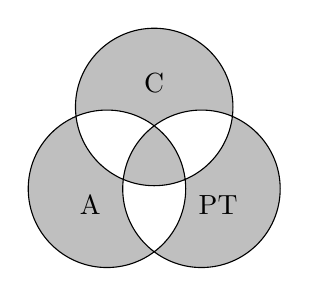
\begin{tikzpicture}
      \filldraw[fill=lightgray,even odd rule]
        (60:1.2) circle (1) ++(90:0.3) node{C}
        (0:0) circle (1) ++(225:0.3) node{A}
        (0:1.2) circle (1) ++(315:0.3)node{PT};
    \end{tikzpicture}
  \end{center}
  \fontsize{6}{8}\selectfont
  Began as a conjecture by Eric Brewer in 2000, being proven by Seth Gilbert
  and Nancy Lynch of MIT in 2002.\\
\end{frame}

\begin{frame}{The Big Picture}
  \framesubtitle{Consistency model revised}
  \begin{description}
    \item[ACID] (traditional, pesimistic - Consistency) \hfill
    \begin{enumerate}
      \item Atomicity
      \item Consistency
      \item Isolation
      \item Durability
    \end{enumerate}
    \item[BASE] (optimistic - Availability + Partition tolerance) \hfill
    \begin{enumerate}
      \item Basically Available
      \item Soft state
      \item Eventual consistency
    \end{enumerate}
  \end{description} 
\end{frame}

\begin{frame}{The Big Picture}
  \framesubtitle{Considering BASE}
\end{frame}

\subsection{The NoSQL Movement}
\begin{frame}{The NoSQL Movement}
  \framesubtitle{What the hell is that? I want my SQL!}
\end{frame}

\end{document}
